\begin{table}[tbp]
\centering
\caption{Held-out winter performance under the common objective. Cost and terminal penalty are daily means in EUR/day; latency shows the controller-call mean and mean daily P95. The offline row averages independently selected five-restart batches when repeated batches are available. CM denotes conditional mean; stochastic MIQP uses two scenarios. The price rule is validation-tuned.}
\label{tab:confirmatory}
\small
\begin{tabularx}{\linewidth}{r>{\raggedright\arraybackslash}Xrrr}
\toprule
Fee & Method & Cost & Terminal & Latency (ms) \\
(EUR/h) & & (EUR/day) & penalty & mean/P95 \\
\midrule
20 & No storage & 1315.3 & 0.00 & 0.0/0.0 \\
 & Price rule & 1315.3 & 0.00 & 0.0/0.0 \\
 & Envelope MPC & 1315.2 & 0.07 & 60.1/123.7 \\
 & CM MIQP & 1248.0 & 2.45 & 416.1/1133.6 \\
 & Stochastic MIQP & 1243.5 & 0.83 & 1174.5/2939.0 \\
 & Offline procedure & 1258.2 & 0.24 & 3.1/3.8 \\
\addlinespace
40 & No storage & 1750.6 & 0.00 & 0.0/0.0 \\
 & Price rule & 1750.6 & 0.00 & 0.0/0.0 \\
 & Envelope MPC & 1750.6 & 0.10 & 53.9/113.3 \\
 & CM MIQP & 1464.8 & 4.20 & 1047.1/2500.0 \\
 & Stochastic MIQP & 1456.0 & 1.74 & 1933.3/4494.0 \\
 & Offline procedure & 1489.1 & 0.37 & 3.1/3.5 \\
\addlinespace
80 & No storage & 2621.3 & 0.00 & 0.0/0.0 \\
 & Price rule & 2621.3 & 0.00 & 0.0/0.0 \\
 & Envelope MPC & 2621.3 & 0.20 & 51.3/110.5 \\
 & CM MIQP & 1782.2 & 5.69 & 1701.3/4425.3 \\
 & Stochastic MIQP & 1746.1 & 3.38 & 2759.2/4989.3 \\
 & Offline procedure & 1769.7 & 0.42 & 3.0/3.4 \\
\bottomrule
\end{tabularx}
\end{table}

\begin{figure}[t]
\centering
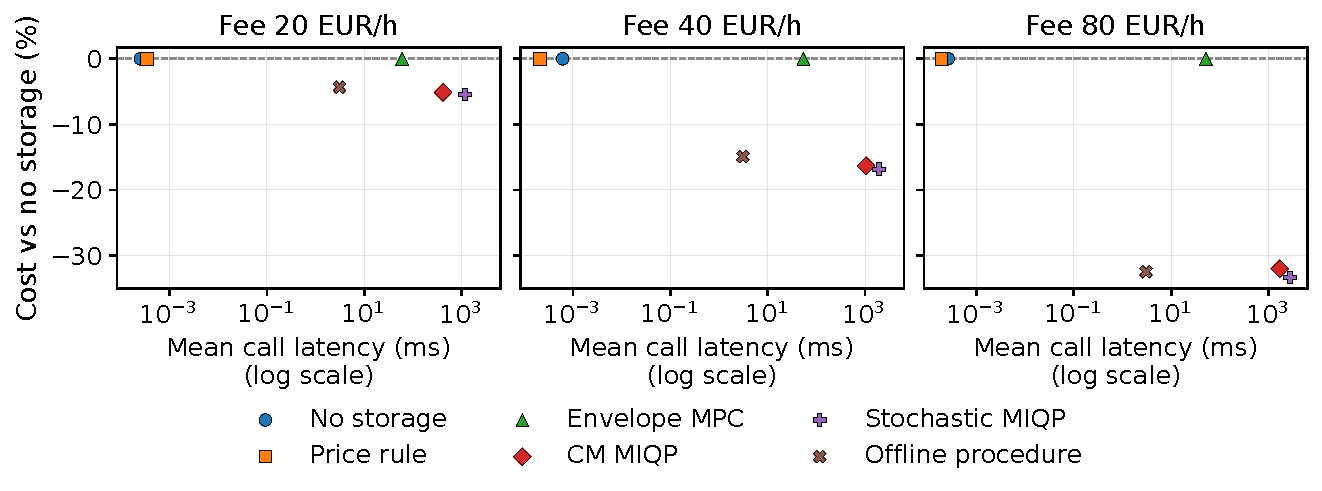
\includegraphics[width=\linewidth]{figures/fig_cost_latency.pdf}
\caption{Operating cost and online computation under the common benchmark. Cost is relative to no storage; latency is measured from controller call to returned held action. Learned evaluation uses the GPU; each MIQP solve uses one CPU thread.}
\label{fig:cost-latency}
\end{figure}

At fee rates of 20, 40, and 80 EUR/h, the offline procedure averaged 1258.2, 1489.1, and 1769.7 EUR/day. These costs were 1.2\%, 2.3\%, and 1.4\% higher, respectively, than the primary two-stage stochastic MIQP (Table~\ref{tab:confirmatory}). The prespecified learned-superiority rule was met in 1 of six MIQP comparisons (Table~\ref{tab:paired}); the supplement reports all baseline comparisons.
The five validation-selected central-fee batch policies ranged from 1485.1 to 1501.1 EUR/day on the common test days.
Zero action was retained in 0 of 7 learned-selection batches. The price-rule baseline selected zero action at all three fees.

A complete five-restart batch required 23.5 minutes of recorded training, validation, and checkpoint loading. Mean online call latency was 3.1 ms, versus 1054.9 ms for conditional-mean MIQP (Figure~\ref{fig:cost-latency}).

\begin{table}[tbp]
\centering
\caption{Primary MIQP comparisons. Differences and bounds are learned minus comparator in EUR/day; fee rates are in EUR/h. The one-sided 95\% upper bound uses paired circular date blocks and, at the central fee, complete training batches. Superiority requires a negative upper bound. Holm $p$ adjusts all 15 comparisons.}
\label{tab:paired}
\small
\begin{tabularx}{\linewidth}{r>{\raggedright\arraybackslash}Xrrrr}
\toprule
Fee & Comparator & Difference & Relative & Upper bound & Holm $p$ \\
\midrule
20 & CM MIQP & 10.3 & 0.8\% & 13.6 & 1.000 \\
20 & Stochastic MIQP & 14.7 & 1.2\% & 17.4 & 1.000 \\
40 & CM MIQP & 24.3 & 1.7\% & 30.3 & 1.000 \\
40 & Stochastic MIQP & 33.1 & 2.3\% & 40.2 & 1.000 \\
80 & CM MIQP & -12.5 & -0.7\% & -6.4 & 0.001 \\
80 & Stochastic MIQP & 23.6 & 1.4\% & 30.1 & 1.000 \\
\bottomrule
\end{tabularx}
\end{table}